\section{Experimentelles Vorgehen und Ergebnisse}

\subsection{Funktionsweise des flouriszierenden Aktinmarkers}
Für die Messung der Aktingeschwindigkeit wurde ein floursizierender Marker verwendet.
Floureszenz beschreibt eine spezielle Art der Abstrahlung von
Photonen durch einen quantenmechanischen Positionswechel
eines Elektron in einen energetisch niedrigeren Zustand.
Für Floureszenz brauch es ein Dreiniveausystem bei dem das
höchste Energieniveau kurzlebig, und das mittlere Energieniveau
sehr langlebig ist. Indem man die passende Lichtfrequenz verwendet,
regt Elektronen in das höchste Energieniveau an, von dem sie sich schnell in das
mittlere Niveau abregen. In diesem Energieniveau verweilen sie, bis es spontan zu einer 
Abregung und der damit verbundenen Lichtemission kommt.
Da die Energiedifferenz zwischen mittlerem und niedrigstem Energieniveau kleiner ist als
die Energiediffernz zwischen dem niedrigsten und dem höchsten Niveau, ist die Wellenlänge
des Abgestrahlten Lichtes kleiner. Das wird schematisch in Abbildung
\ref{fig:dreiniveausystem} verdeutlicht.

\begin{figure}[]
  \centering
  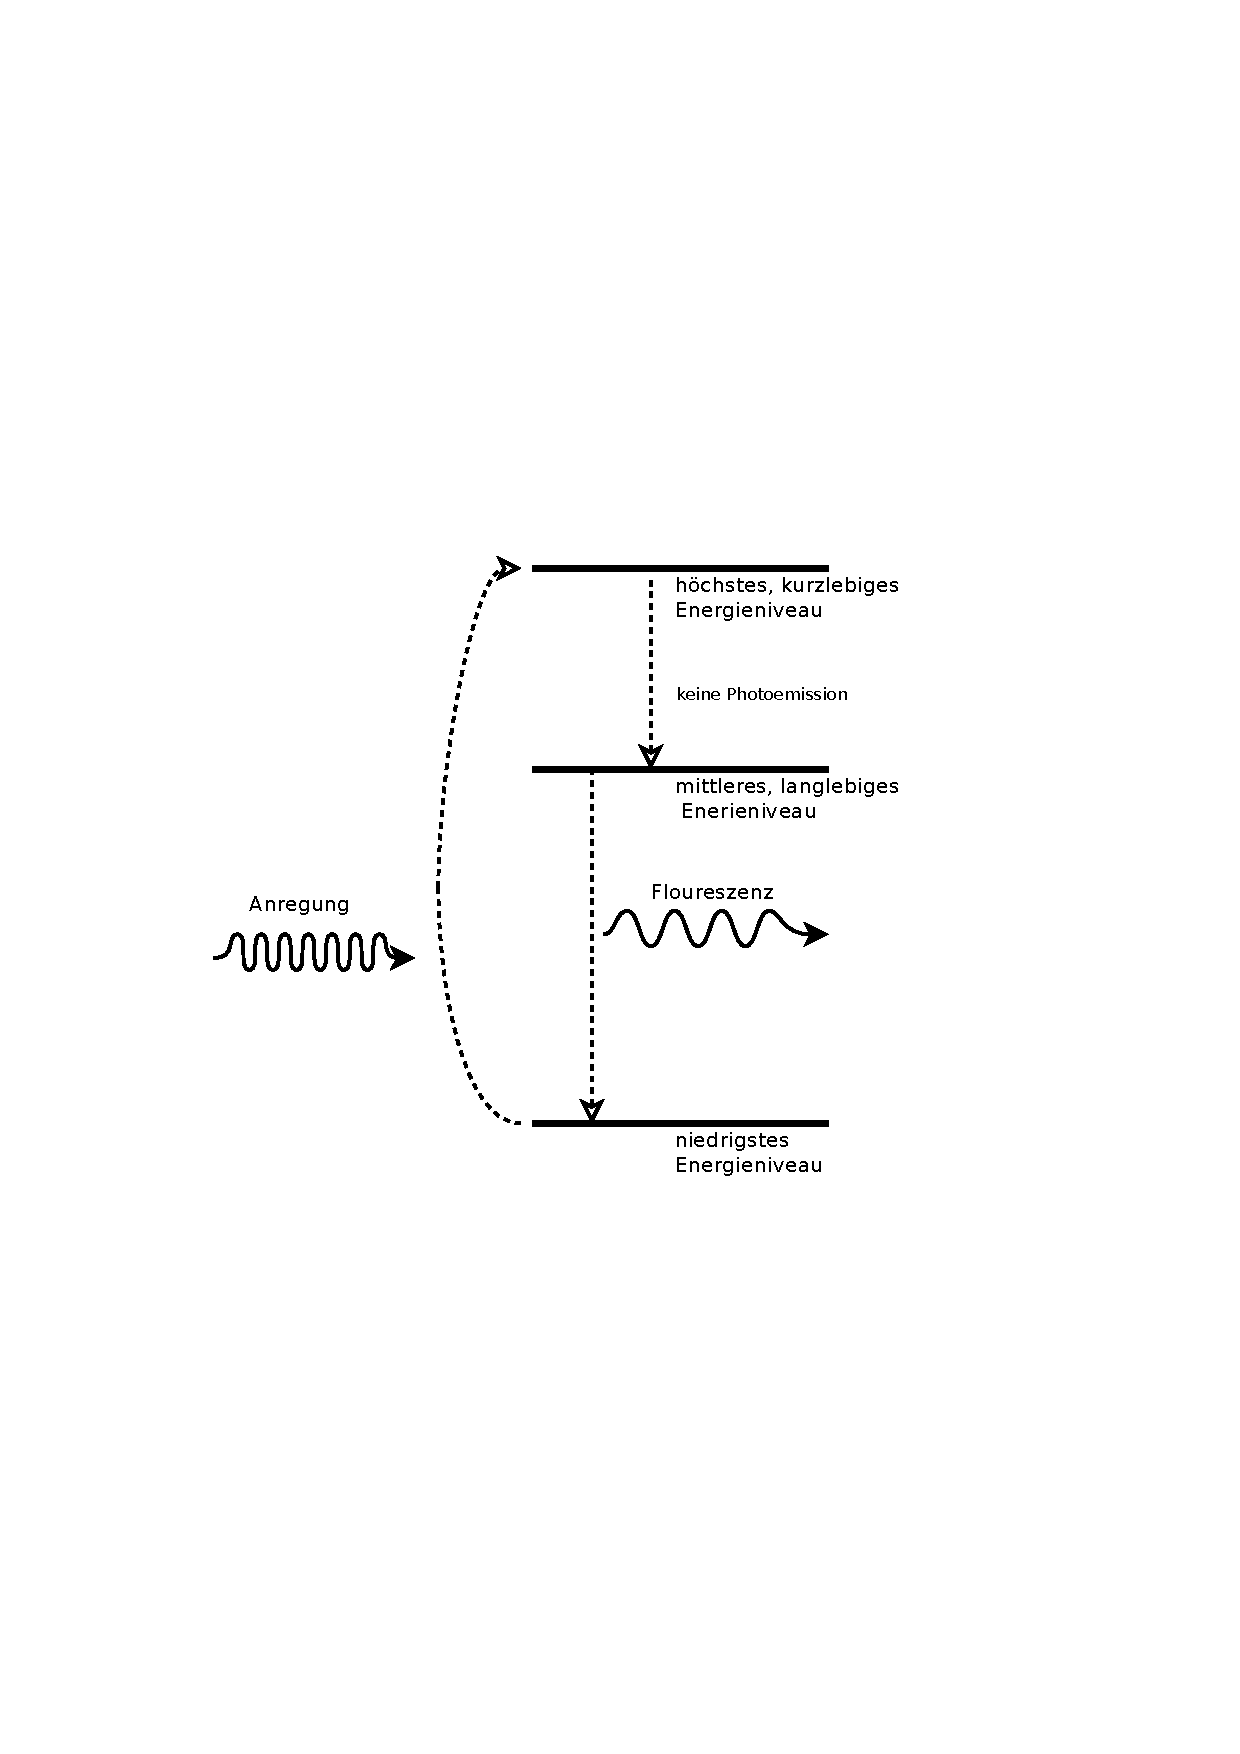
\includegraphics[width=\textwidth]{bilder/energieniveauschema.pdf}
  \caption{Ein Dreiniveausystem für Floureszenz}
  \label{fig:dreiniveausystem}
\end{figure}

\subsection{Zusammenhang zwischen numerischer Apertur und Auflösungsgrenze}
Die Auflösungsgrenze eines Mikroskopes ist durch die numerische Aptertur $N_{A}$ gegeben,
einer dimensionslosen Zahl, die abhängig von der Wellenlänge den minimalen noch zu messenden
Abstand zwischen zwei Lichtpunkten angibt. Der minimale Abstand $d_{min}$ lautet:
\begin{equation}
  d_{min} = \frac{0.61 \lambda}{N_{A}}
\end{equation}
Hätten wir in unserem Versuch ein Auficht, oder ein Druchlichtmikroskop
für die Analyse der Aktingeschwindigkeit verwendet, hätten wie bei blauem
Licht mit $ \lambda = 488nm$ und der im Versuch gegebenen Linse eine
Auflösungsgrenze von 180 nm.

\subsection{Abhängigkeit der Aktingeschwindigkeit von der ATP}
Der flouriszierende Marker ist ein Mo
\begin{figure}[]
  \centering
  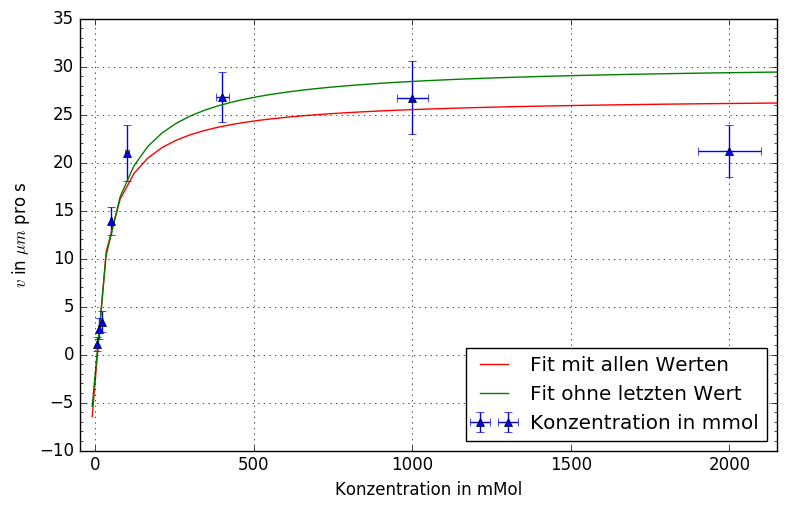
\includegraphics[width=0.8\textwidth]{bilder/both_fits.png}
  \caption{gemessene Aktingeschwindigkeit in $\sfrac{\mu m}{s}$ in A}
  \label{fig:abbe}
\end{figure}


%%% Local Variables:
%%% mode: latex
%%% TeX-master: "../motors"
%%% End:
